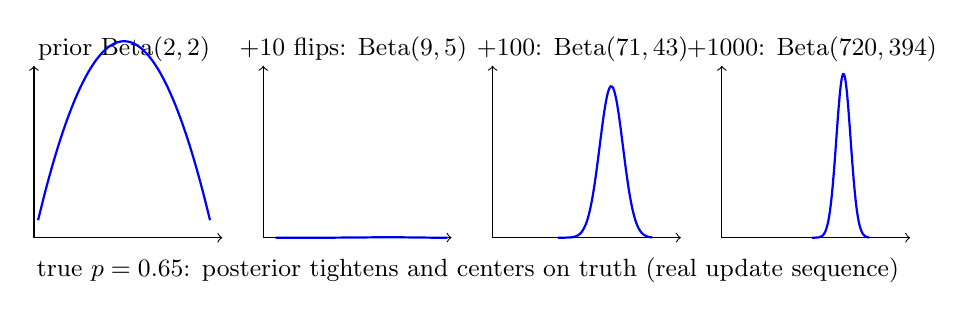
\begin{tikzpicture}[scale=0.52]
% Beta pdf approximations via parabola-ish shapes; Beta(2,2) dome, (9,5) skew right, (71,43) tight, (720,394) needle
\begin{scope}
\node at (2.2,4.6) {\small prior $\mathrm{Beta}(2,2)$};
\draw[domain=0.1:4.3,smooth,thick,blue] plot (\x,{3.2*(\x/4.4)*(1-\x/4.4)*6});
\draw[->] (0,0)--(4.6,0); \draw[->] (0,0)--(0,4.2);
\end{scope}
\begin{scope}[xshift=5.6cm]
\node at (2.2,4.6) {\small $+10$ flips: $\mathrm{Beta}(9,5)$};
\draw[domain=0.3:4.5,smooth,thick,blue,samples=50] plot (\x,{22*((\x/4.6)^8*(1-\x/4.6)^4)});
\draw[->] (0,0)--(4.6,0); \draw[->] (0,0)--(0,4.2);
\end{scope}
\begin{scope}[xshift=11.2cm]
\node at (2.2,4.6) {\small $+100$: $\mathrm{Beta}(71,43)$};
\draw[domain=1.6:3.9,smooth,thick,blue,samples=60] plot (\x,{3.7*exp(-((\x-2.9)^2)/0.16)});
\draw[->] (0,0)--(4.6,0); \draw[->] (0,0)--(0,4.2);
\end{scope}
\begin{scope}[xshift=16.8cm]
\node at (2.2,4.6) {\small $+1000$: $\mathrm{Beta}(720,394)$};
\draw[domain=2.2:3.6,smooth,thick,blue,samples=60] plot (\x,{4.0*exp(-((\x-2.97)^2)/0.06)});
\draw[->] (0,0)--(4.6,0); \draw[->] (0,0)--(0,4.2);
\end{scope}
\node at (10.6,-0.8) {\small true $p=0.65$: posterior tightens and centers on truth (real update sequence)};
\end{tikzpicture}
